% Chapter 8

\chapter[Design]{Design} % Main chapter title

\label{Chapter8} % For referencing the chapter elsewhere, use \ref{Chapter8} 

%----------------------------------------------------------------------------------------

This section describes the design of the system, and gives details of the reasoning behind some of the design decisions. This design work was done largely prior to implementation, with some elements of the design being re-factored during the implementation phase in adherence to the agile development methodology being followed. The design process was broken down into a number of key areas. Firstly the design of the software architecture, including the breakdown of the different components and the path of data through the system. This served as a road map during the implementation stage. The second key area was the user interface design. This involved determining how the main application should appear to the user, how best to provide the user with access to the various features, and then creating a template of the window and component layout required to achieve this. Graphical representations were also designed for each of the data types to be displayed in the visualiser.

%----------------------------------------------------------------------------------------

\section{Software Architecture Design} \label{SoftwareArchitectureDesign}
The guiding principles of the software architecture design were `Object Oriented Programming' (OOP) practices, and the `model-view-controller' (MVC) software architecture pattern. OOP \cite{OOP} is an extremely widespread concept in modern software development theory. It states that code should be organised into units based on individual functionalities, commonly referred to as classes. Each class collects together the data that describes an object and the routines to perform actions with and on that data. A class then acts as a template, and a new instance of the class can be instantiated each time an object of that type is needed. OOP aims to make code easier to understanding and maintain, reduce code duplication, and increase re-usability and modularity. Designing software in an OOP fashion is standard practice for most modern programming tasks, and modern languages are often designed around OOP concepts.

C++ was selected as the development language for this application as it offers much of the low level control and efficiency of the C language, whilst also supporting OOP practices natively. The majority of the existing software infrastructure in the YRL had also been implemented in C++, hence following suit would help with maintainability and integration in the future. Considering the project's requirements for interfacing with low level hardware such as the tracking camera (via a driver) and the robots (via network sockets), and for performing image processing, the speed and low level capabilities of C++ also seemed beneficial. Higher level languages such as Java were considered, as they offered a number of different benefits such as better portability and automatic resource management, but were ultimately deemed less suitable.

The MVC software architecture design pattern is another widespread concept in software development theory. It primarily relates to the programming of applications with user interfaces. The three words that give the pattern its name - model, view and controller - define the three 'layers' into which code components are organised. The model refers to the application's data, and includes all of the information that defines an application's current state. The view refers to the code used to produce the user interface from the data in the model layer. It acts as the method by which the user 'views' the data, thus getting its name. Finally the controller layer acts as the intermediary between the two, retrieving data from the model and processing it if necessary before passing it to the view for display. The controller also responds to input and changes the data in the model accordingly. This includes data input via the user through the view, as well as data from other sources. In the case of this application these other sources include the peripherals, such as the tracking camera, and the robots via the WiFi network. Adhering to an MVC pattern helps to keep code structured and organised, making it easier to understand, maintain and extend. It ensures that state data is not maintained or duplicated within the UI code, and that only one, true copy of the application data exists, stored in the model layer.

With these two principles in mind, the software design process could begin. First the application was broken down into individual components based on the functional specification. The following key areas were identified:

\begin{itemize}
\item Code to handle communicating with the camera and retrieving the image data.
\item Code to perform the robot tracking.
\item Code to handle the networking, including receiving data from the robots.
\item Code defining a model to store the robot data in.
\item Code to enter new data into the model.
\item Code to augment the video feed based on the stored data.
\item Code to display the video and augmentations feed to the user.
\item Code to respond to user input via the user interface
\item Code to store user settings
\end{itemize}

\begin{figure}
	\centering
	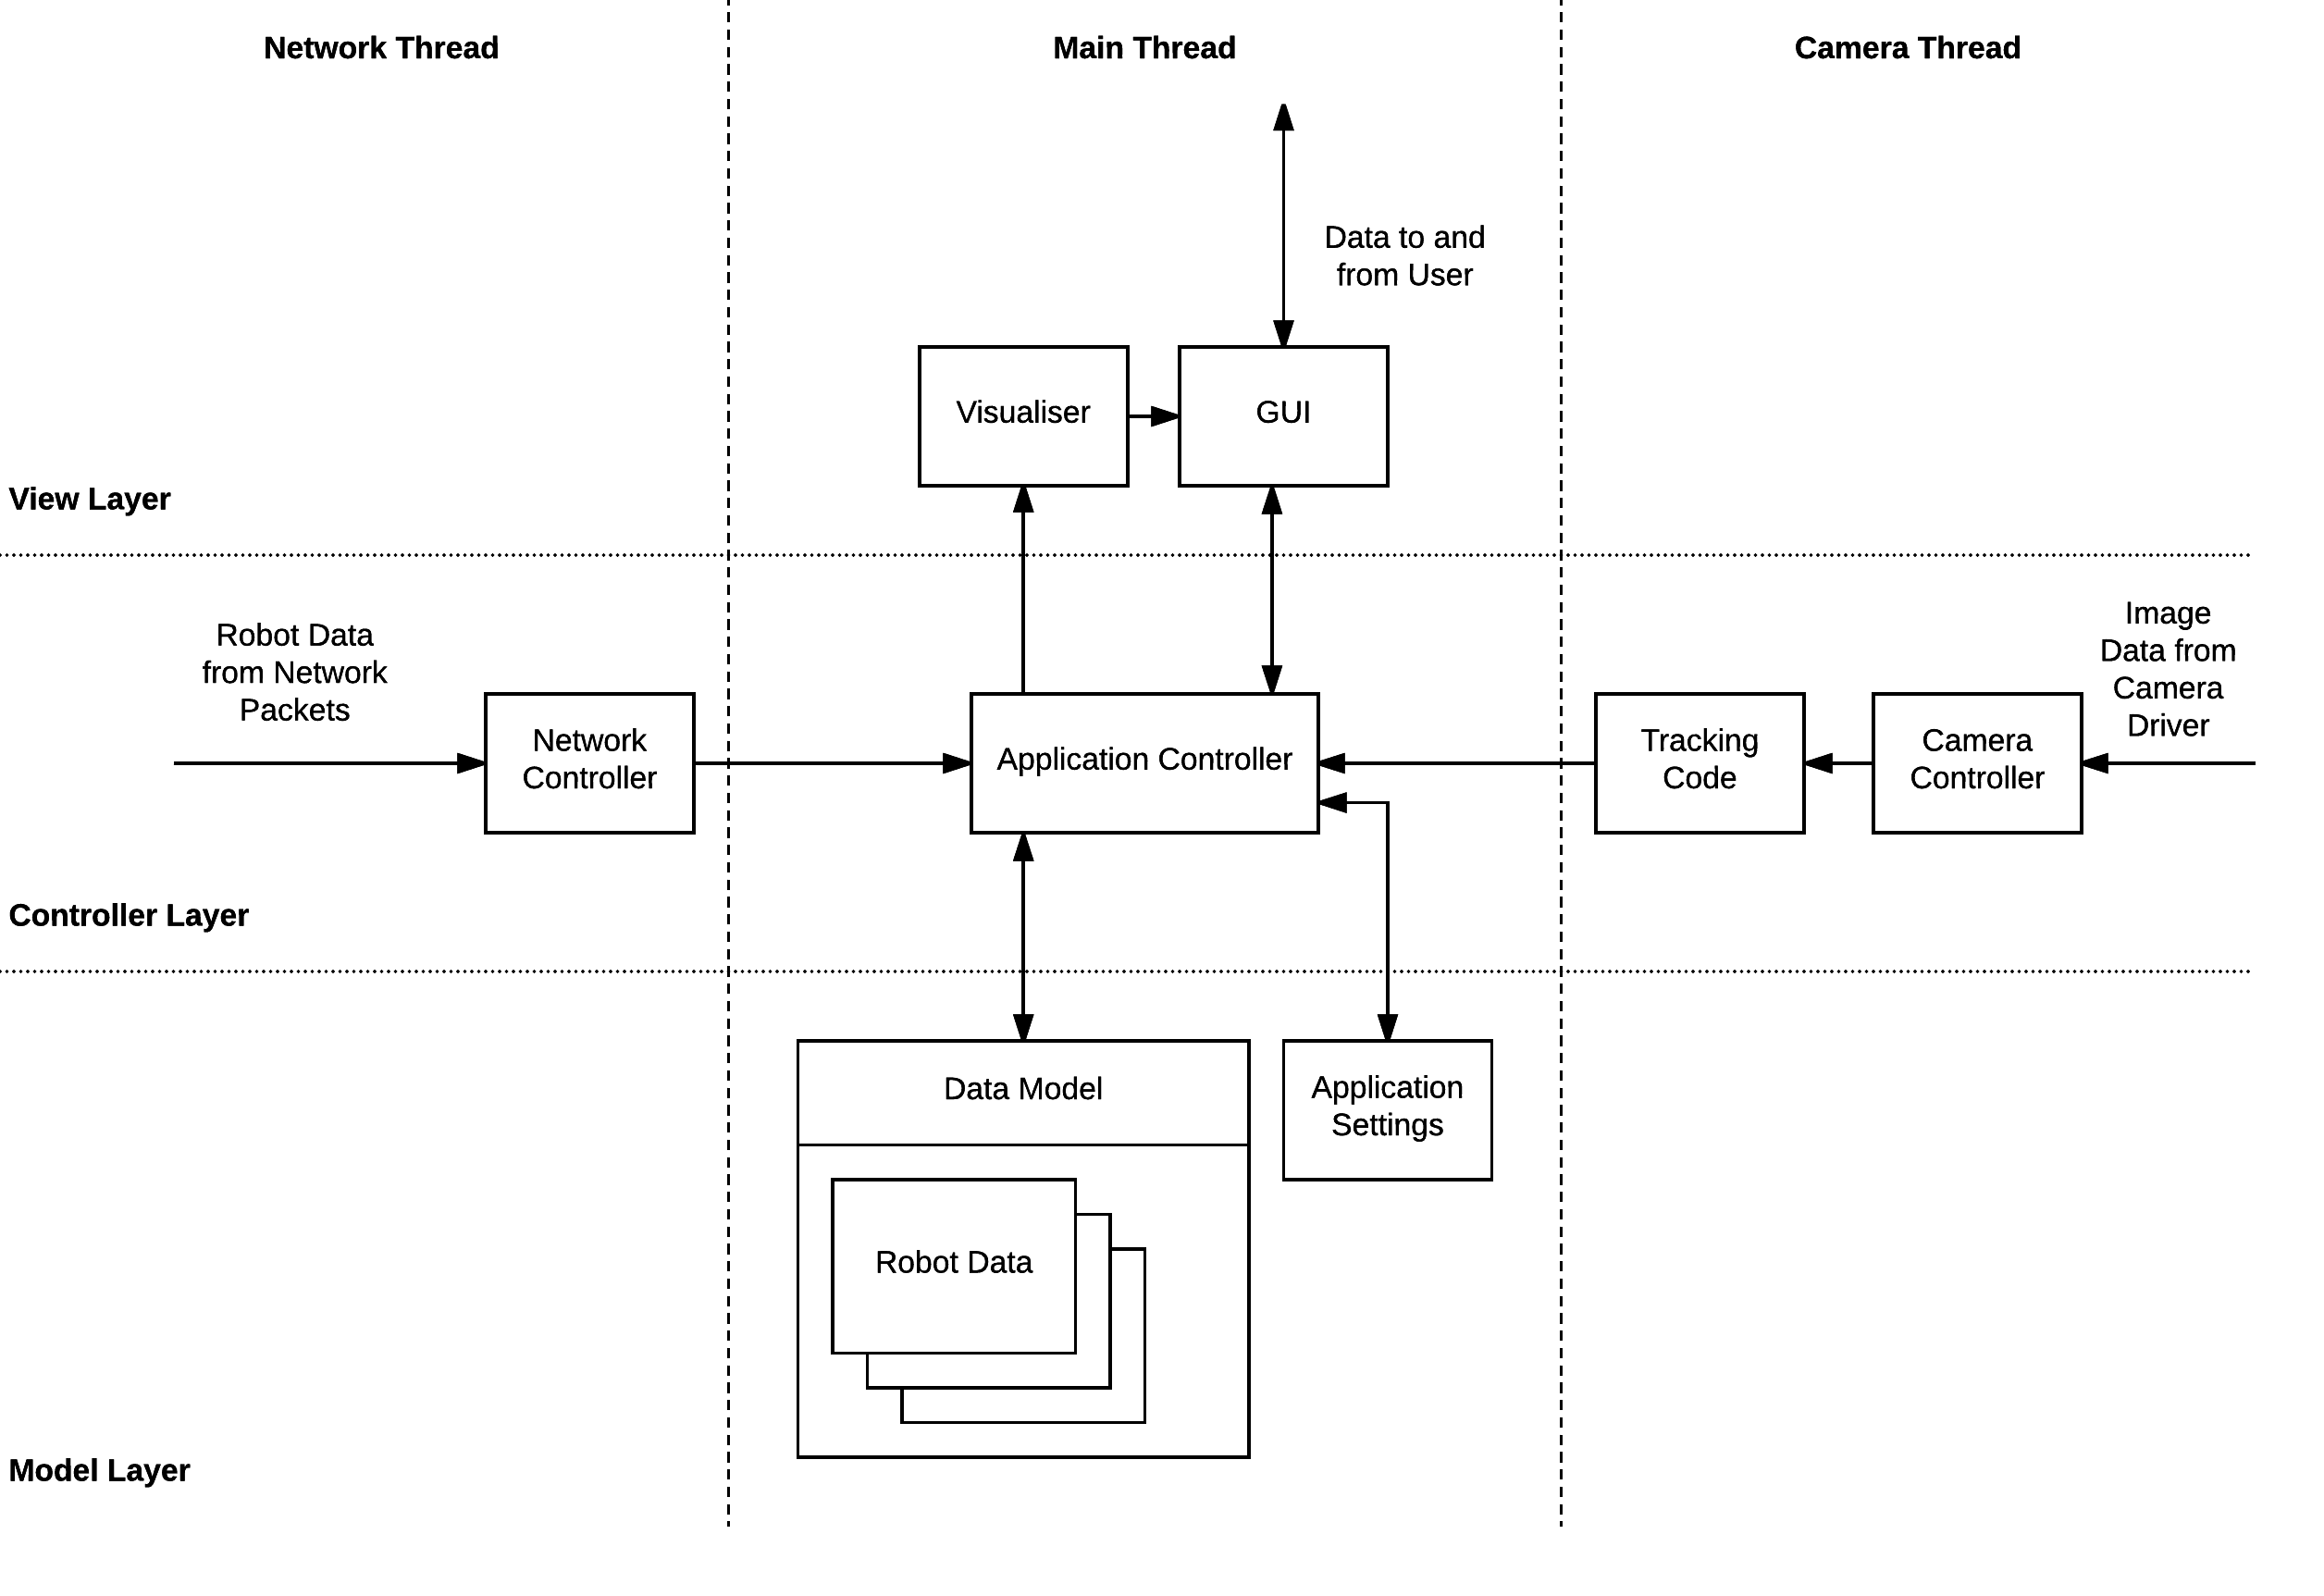
\includegraphics[scale=0.7]{Figures/SoftwareArchitecture.png}
	\decoRule
	\caption[Software Architecture Diagram]{A diagram of the software architecture design and data flow.}
	\label{fig:SoftwareArchitecture}
\end{figure}

Once separated into functional components, the required code blocks could be organised into a structure, and the data path of the application examined. Figure \ref{fig:SoftwareArchitecture} shows this structural arrangement, with boxes for each of the functional objects and arrows indicating data flow. The three layers of the MVC design pattern are shown by the vertical partitioning. The horizontal partitioning is used to show another key design consideration - threading. In order to maximise performance and ensure responsiveness, functionality which has the potential to `block' execution whilst waiting for a result or response should be run in a separate thread. This application was therefore designed with three threads in mind. The main thread handles the core of the application, including all data model access and GUI operations. The network thread handles communicating with the robots via WiFi. It was anticipated that this networking would involve low level socket code, which meant the potential for blocking socket-read operations, therefore requiring a separate thread. The camera thread handles reading the machine vision camera and performing the tag tracking using the ArUco library. It was anticipated that the camera read operation could block until the next frame was available in the camera driver's buffer. Tracking the robots in the image using the ArUco library also had the potential to be CPU intensive, so keeping this off the main thread was considered a potential performance benefit.

As can be seen in figure \ref{fig:SoftwareArchitecture}, the software architecture is structured around a central application controller. The data from all other components of the application flows through this central component, which routes it to where it needs to go. It is also responsible for updating the visualiser and GUI with new data when necessary, and acting on the user input signals received through the UI. The other key controller layer components - the network controller and the camera controller - exhibit data flow in only one direction. The design of these components was therefore relatively simple, as they needed only to perform the following loop of tasks:

\begin{enumerate}
 \item Receive data from external source.
 \item Process data as necessary, extracting required information.
 \item Notify the application controller of the newly available data.
 \item Wait for new data to become available.
\end{enumerate}

The remaining components are more complex, and required greater software design considerations. The design of the data model is discussed in section \ref{DataModelDesign}. The design of the visualiser code is discussed in section \ref{VisualiserDesign}.

\subsection{Data Model} \label{DataModelDesign}
\begin{figure}[h]
	\centering
	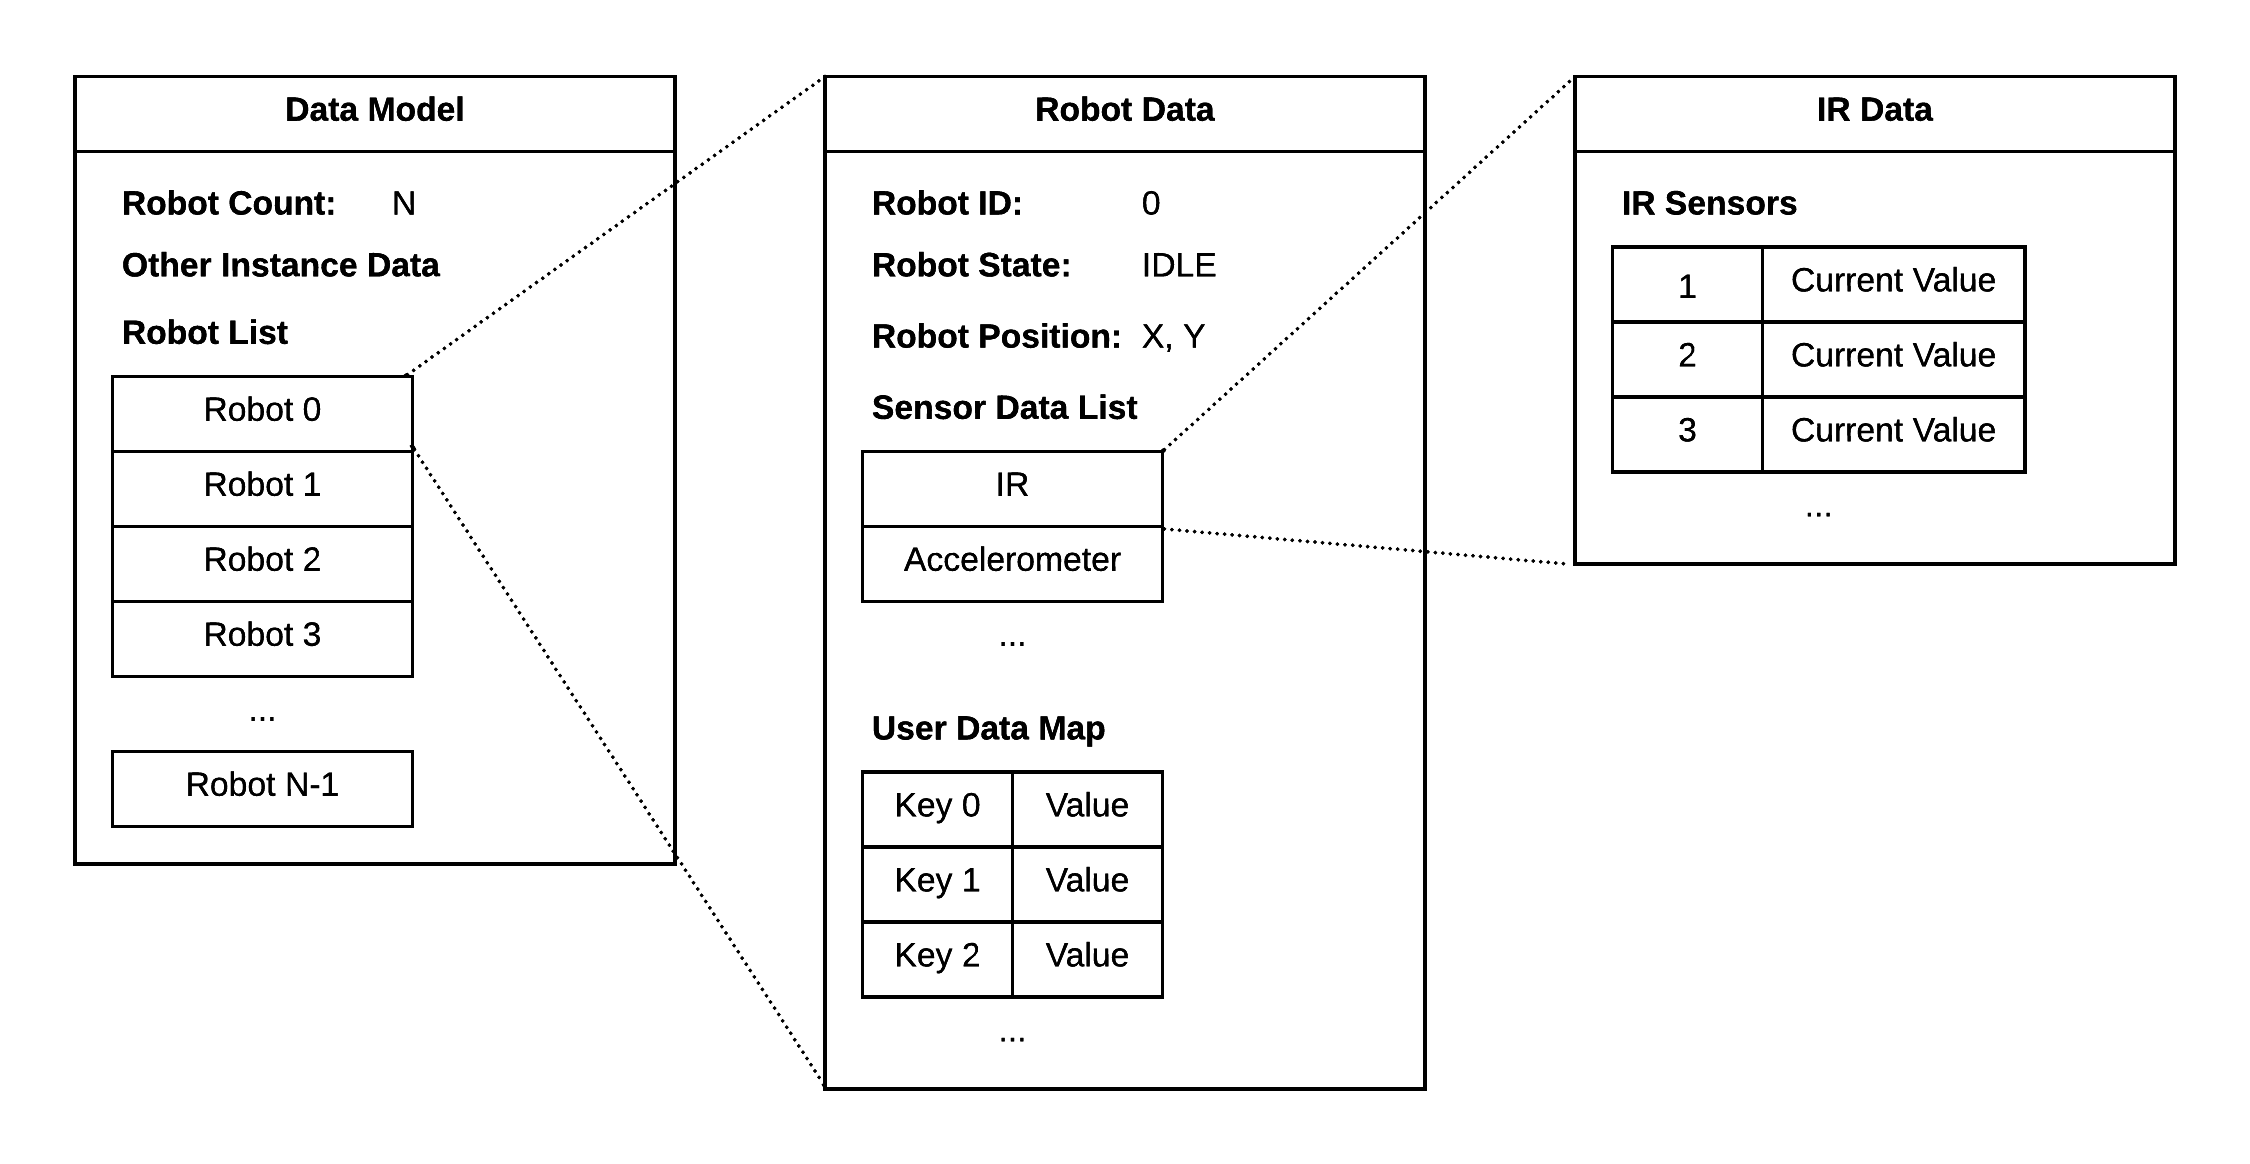
\includegraphics[scale=0.7]{Figures/DataModel.png}
	\decoRule
	\caption[Data Model Diagram]{A diagram of the data model design.}
	\label{fig:DataModel}
\end{figure}

The purpose of the data model component is to store all of the data required to describe the applications current state. This includes all data related to each of the robots being tracked by the system. In order to achieve this in an object oriented manner the data model itself was designed to comprise a number of smaller components in a hierarchical structure. The main data model object maintains a collection of smaller objects, each containing the data related to a single robot. These in turn maintain a collection of different data objects relating to the robot's state and sensor data. Figure \ref{fig:DataModel} illustrates this hierarchical data model design using the IR sensor data of a single robot as an example.

This follows object oriented programming practices by defining a single class to describe a robot, from which a new robot data object can be instantiated each time the system begins tracking a new robot. When data is received regarding a robot the system is already aware of, it can simply update the correct existing robot data object with the new data.

\subsection{Visualiser} \label{VisualiserDesign}
\begin{figure}[h]
	\centering
	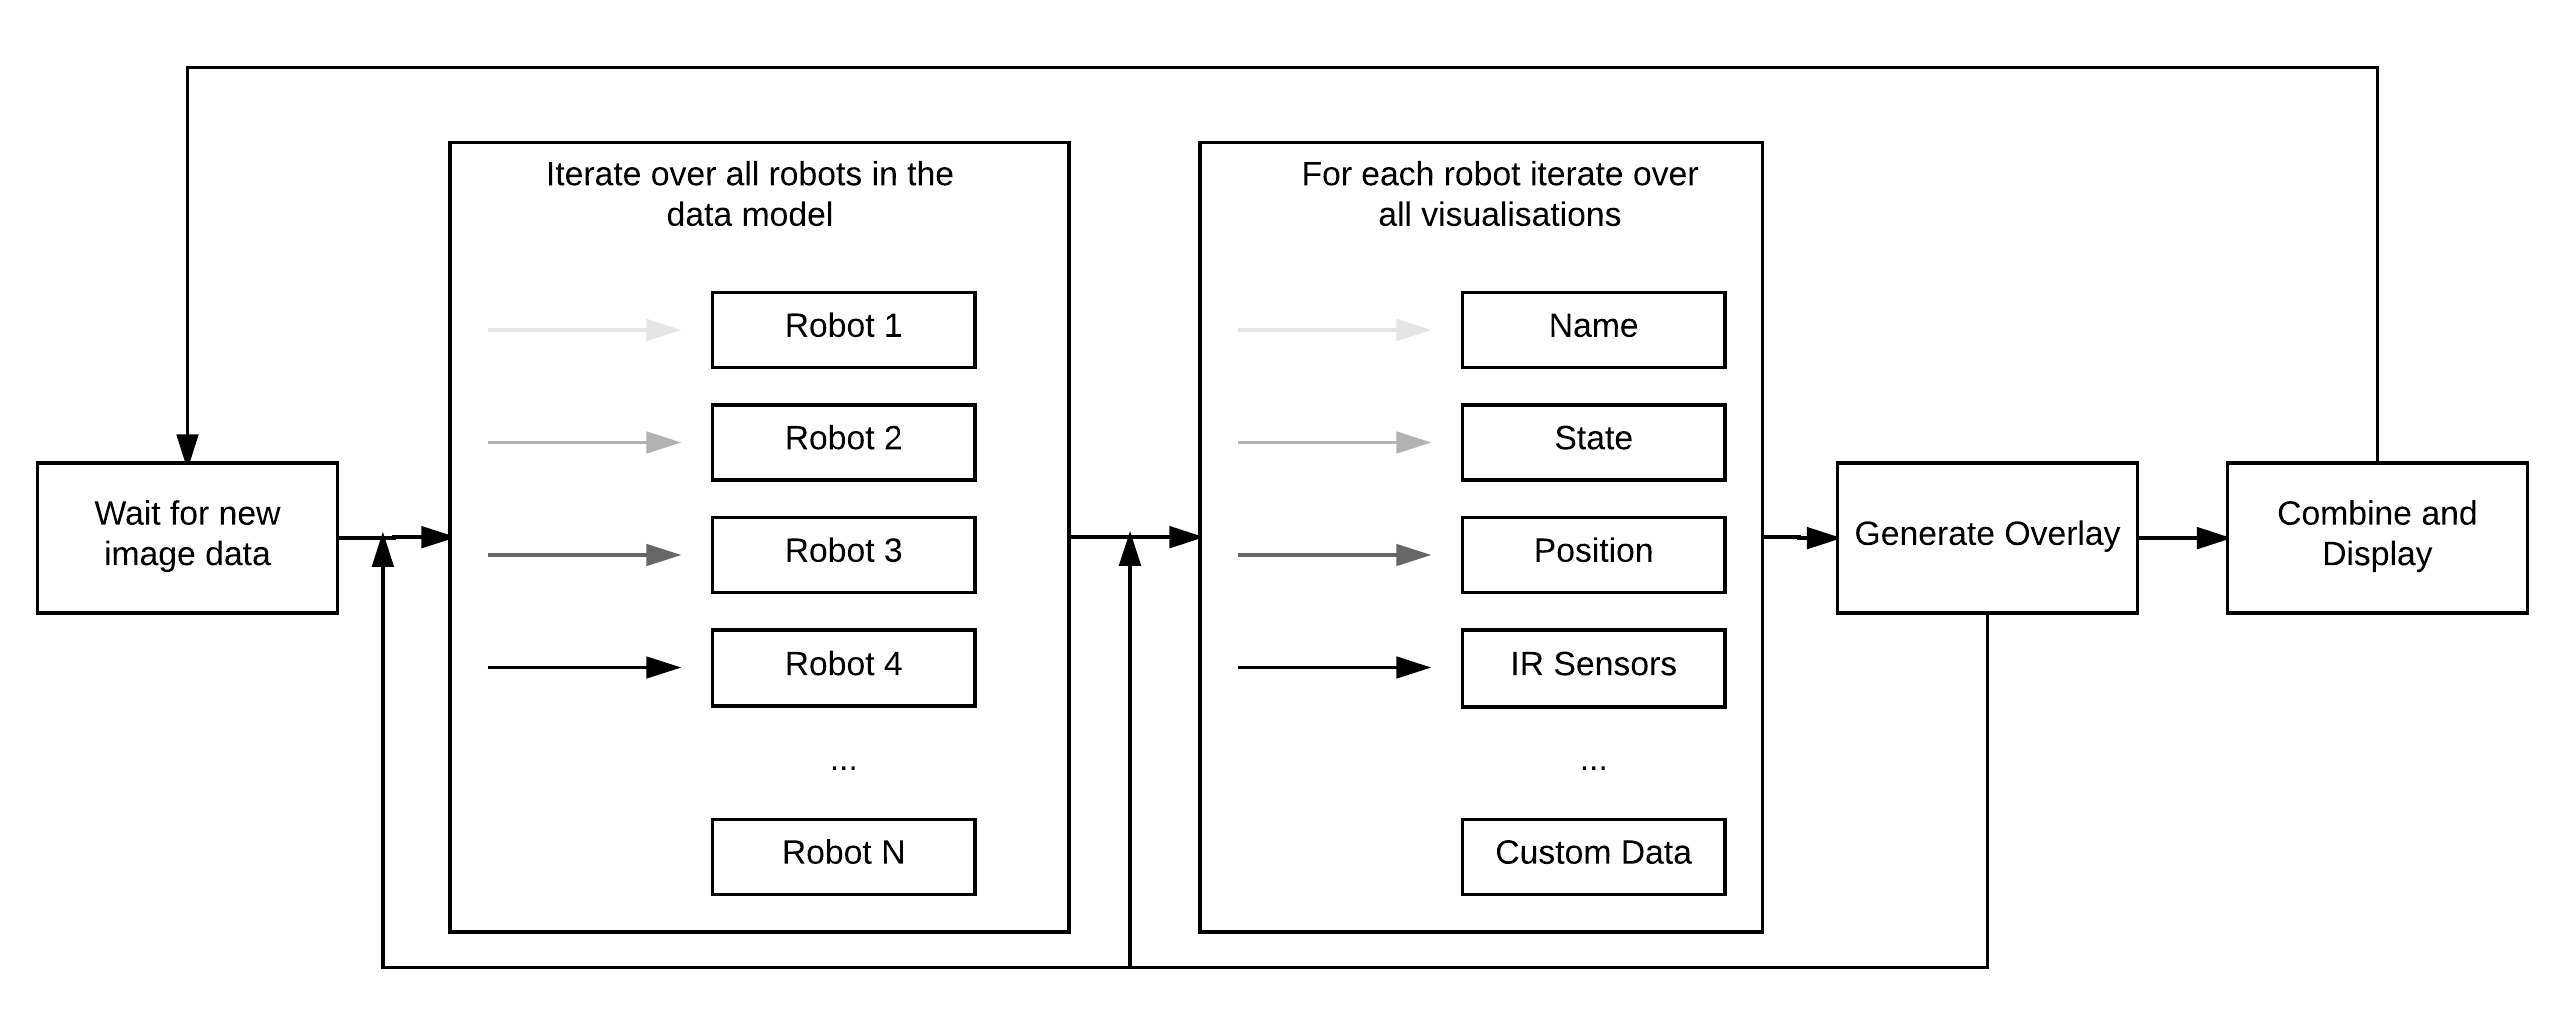
\includegraphics[scale=0.7]{Figures/VisualiserProcess.png}
	\decoRule
	\caption[Visualiser Render Process Design]{A diagram describing the design of the visualiser rendering process.}
	\label{fig:VisualiserProcess}
\end{figure}

The purpose of the visualiser component is to generate and display the augmented video feed to the user. The component therefore receives the latest camera image and the most up to date robot data, generating the graphical overlays based on a combination of the robot data and the current settings for each visualisation. It then displays the latest image, with the graphical overlays applied, to the user by rendering it as a single image within the appropriate GUI element. This rendering process occurs each time a new video frame is read from the camera, hence both the video and the overlays should update regularly and respond rapidly to changes in the robot data.

In order to further modularise the visualiser code, it was broken down into a number of smaller components. For each type of data visualisation a separate component was defined, which describes how the visualisation for that data type is generated, based on a single robot data object. The main visualiser component could then be designed to generate the graphical overlays iteratively, by stepping through the available set of robot data objects, and for each one step through the different visualisation components, generating the overlay for each combination. The overlays can then be combined and displayed as a single image. Figure \ref{fig:VisualiserProcess} describes this process diagrammatically.

%----------------------------------------------------------------------------------------

\section{User Interface Design} \label{UserInterfaceDesign}
\begin{figure}[h]
	\centering
	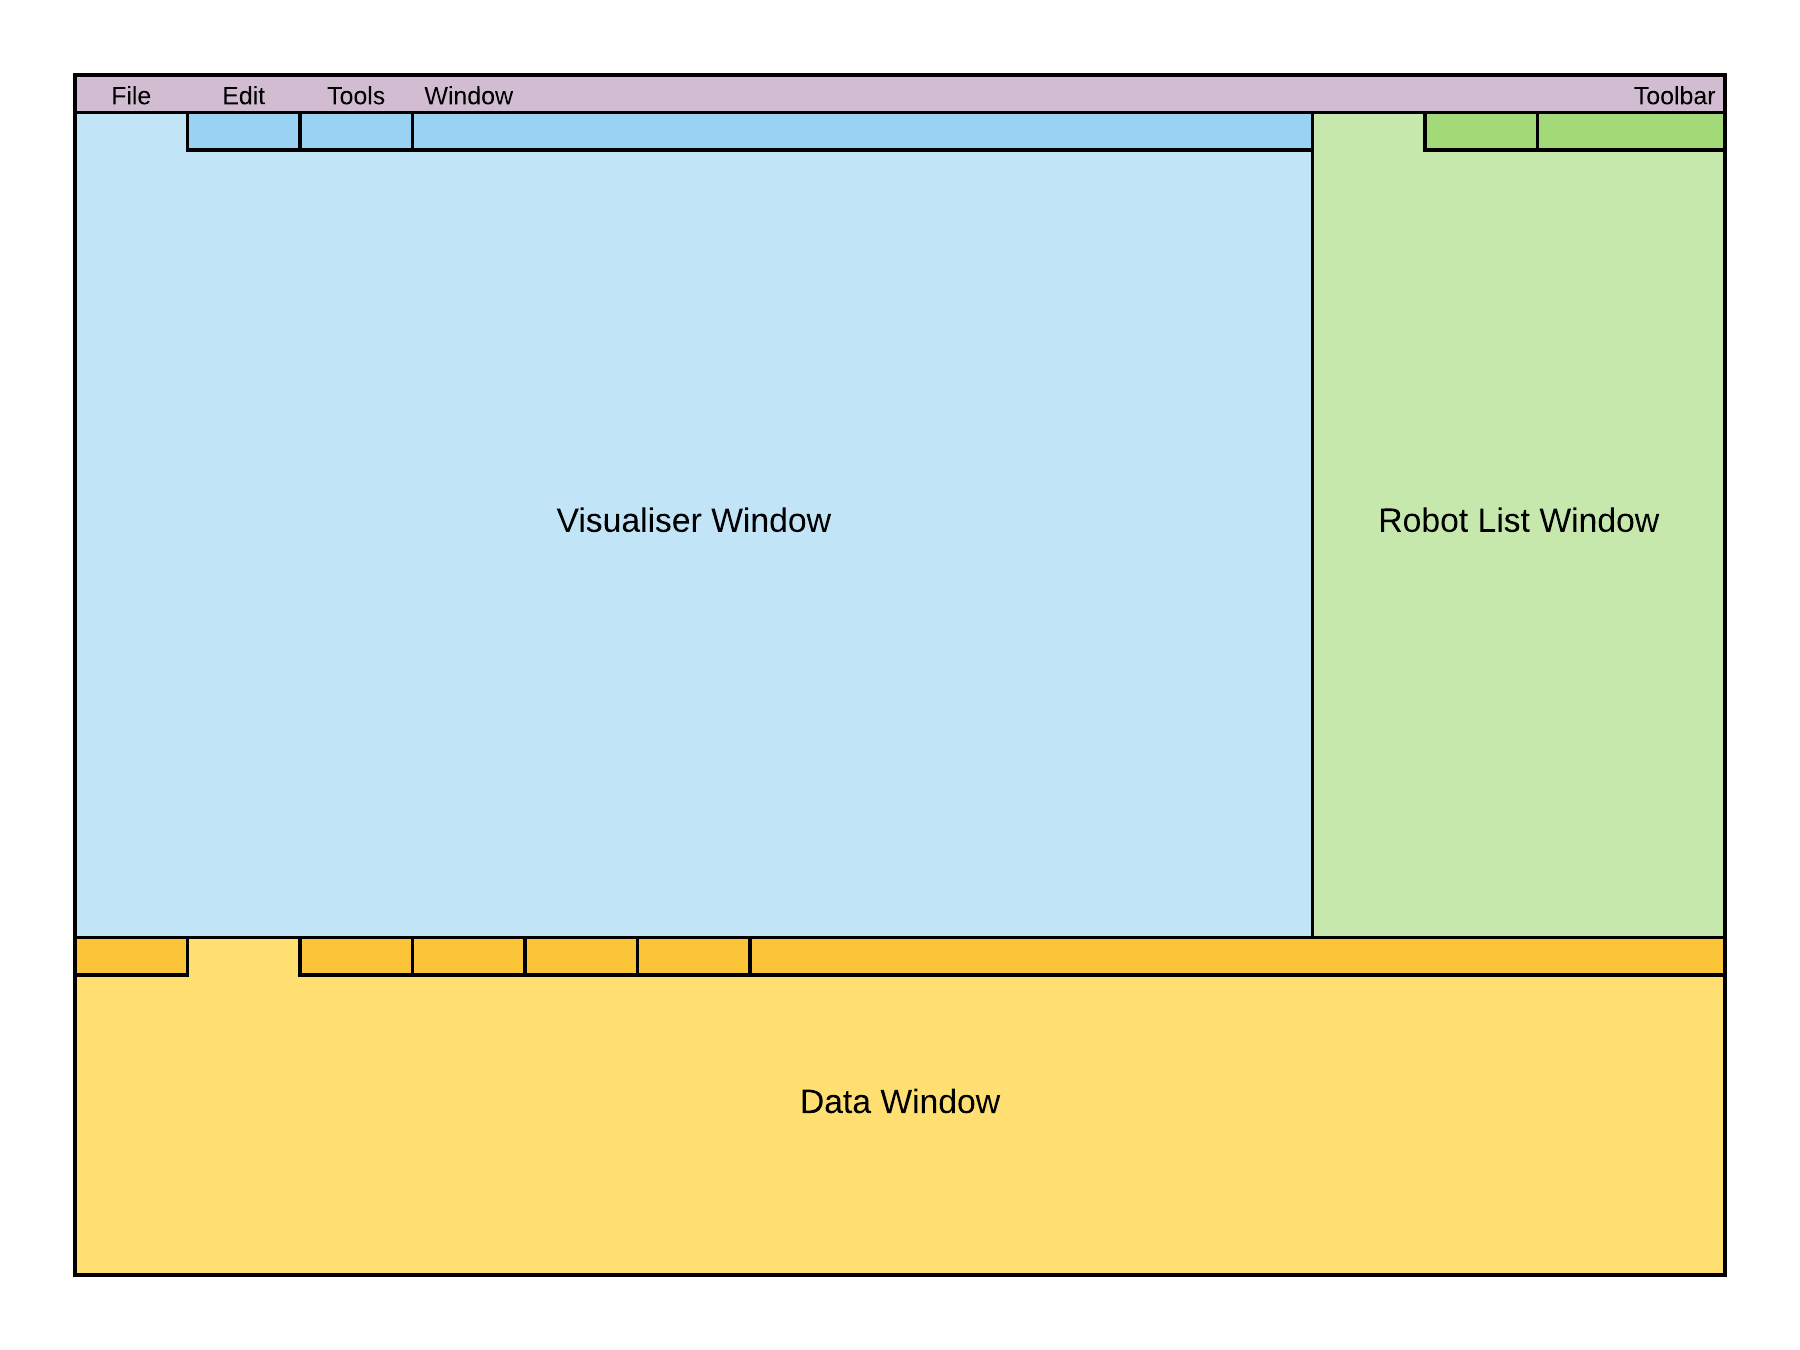
\includegraphics[scale=1]{Figures/UILayout.png}
	\decoRule
	\caption[UI Layout]{The design of the basic user interface layout.}
	\label{fig:UILayout}
\end{figure}

The second main area of consideration during the design phase was the Graphical User Interface (GUI). It was determined that creating a well designed, intuitive interface would be essential to satisfying the objective of providing data in a 'human readable' form. Having real time data would be useless if the user cannot parse the data displayed sufficiently quickly, due to a poorly designed or confusing UI. The first decision made was to try and keep the interface familiar to a computer user, through the use of standard, widely understood user interface elements. There exists a well defined `language' in computer interface design, using constructs such as windows, panels, tabs, buttons, text fields and other elements which have well understood functions. It was thought that basing the user interface design on this well established standard would minimise the time for a new user to become accustomed to the system. The next step was determining how many panels would be necessary for the intended functionality to be possible, and how best to lay these out within the window and organise the smaller elements within each panel. Three main panels were determined to be necessary. The first would display the video feed and visual overlay, the key component of the application. A second panel would be used to display a list of the robots known to the system, so that they could be selected without obscuring the visualiser. Finally a third panel would be used to display more detailed information about the selected robot in a number of different tabs. Figure \ref{fig:UILayout} shows the basic layout design for these main panels.

The visualiser panel, highlighted in blue, takes primary place in the layout. In order to maximise the readability of the augmented video feed it was determined that this panel should occupy as much space as possible. A number of tabs allow the user to change the focus of the panel, giving access to various settings, including settings for the visualiser and camera. The robot list panel is highlighted in green on the right hand side. This requires less width, as it's main function is to display a list of the known robots, and allow the user to select one. Again tabs within the panel allow the user to access functionality related to the robots, such as settings for the network connection. Finally the data panel is highlighted in yellow at the bottom of the layout. Each of the tabs provide more detailed info on a specific type of data collected about the selected robot, as well as a tab for a general overview, and a console-style log of application events. It was noted that when displaying data in this panel it should be formatted to maximise the use of the available space. This means using the full width of the window and limiting the height to avoid excessive scrolling. The design also includes a toolbar at the top of the window, another standard feature of window-based software applications. The toolbar is provided to allow quick access to useful functionalities.

\begin{figure}[h]
	\centering
	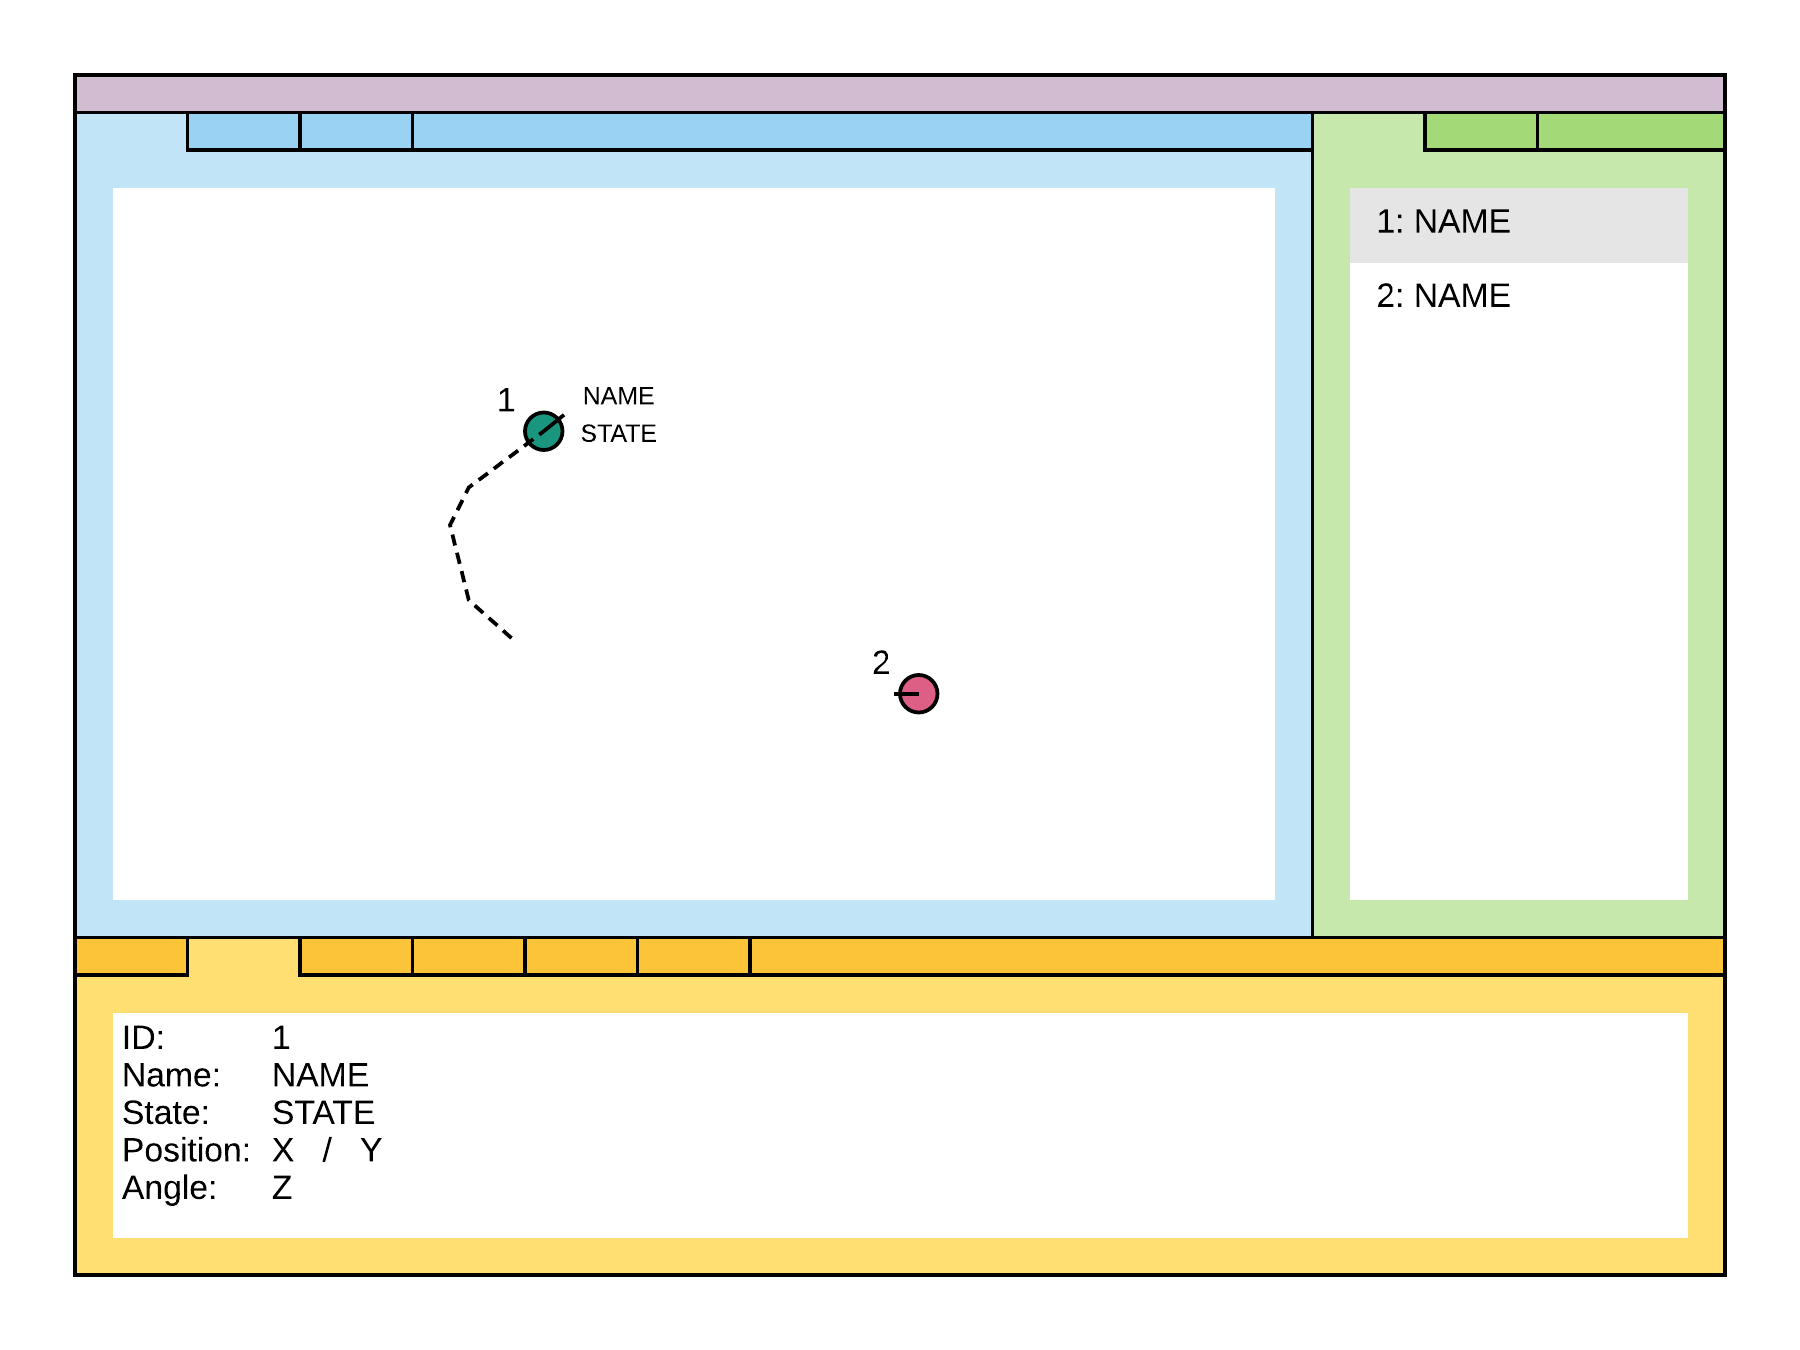
\includegraphics[scale=1]{Figures/UIExample.png}
	\decoRule
	\caption[UI Example]{The basic UI design, filled with some example content.}
	\label{fig:UIExample}
\end{figure}

Figure \ref{fig:UIExample} shows how this layout might look when filled with some example content. The robot list identifies the two robots being tracked by the system, and shows that robot 1 is selected. The visualiser component shows an example of how the video image might be augmented with graphical overlays generated from data regarding the two robots. These overlays include indicators for each robots position and orientation, as well as text showing the name and state of the selected robot. The dotted line shows the recent path taken by the robot, which is an example of one potential type of data visualisation. Colour is also used to differentiate the two robots. The data view at the bottom of the window shows some example data for the selected robot, which might be seen on a general `overview' tab.

Time was also spent creating more detailed designs for some of the individual tabs within the main panels. Each tab within the data panel needed to display a different data type, and therefore required a unique layout and design. Figure \ref{fig:DataPanelDesigns} shows the initial designs for four of the key tabs, using both textual and graphical approaches to data representation. Layout 1 shows the overview tab design, as seen previously. Layout 2 shows the design for the console tab, which displays messages about the application sequentially. Layout 3 shows the state tab, which offers additional information about the state of the selected robot, beyond simply its current state. The first box displays a list of all of the robot's known states, and the second box displays a list of the robot's recent state transitions, including the original state, the new state and the time the transition occurred. Finally layout 4 shows one possible design for displaying the robot's IR sensor data, using a bar graph to give a relative, comparable impression of each sensors value, and the numerical displays beneath to provide the actual sensor values. Figure \ref{fig:VisualiserSettingsTabDesign} shows the design for the settings tab of the visualiser panel. The purpose of this tab is to provide access to general settings related to the visualiser, and specific settings for each of the data visualisation types. The actual settings shown in the design are representative. General settings are changed using basic form controls such as tick boxes. Settings for specific visualisations can be changed using extra pop-up windows accessed by double clicking the relevant visualisation in the list. In figure \ref{fig:VisualiserSettingsTabDesign} the IR data visualisation settings are shown as an example.

\begin{figure}
	\centering
	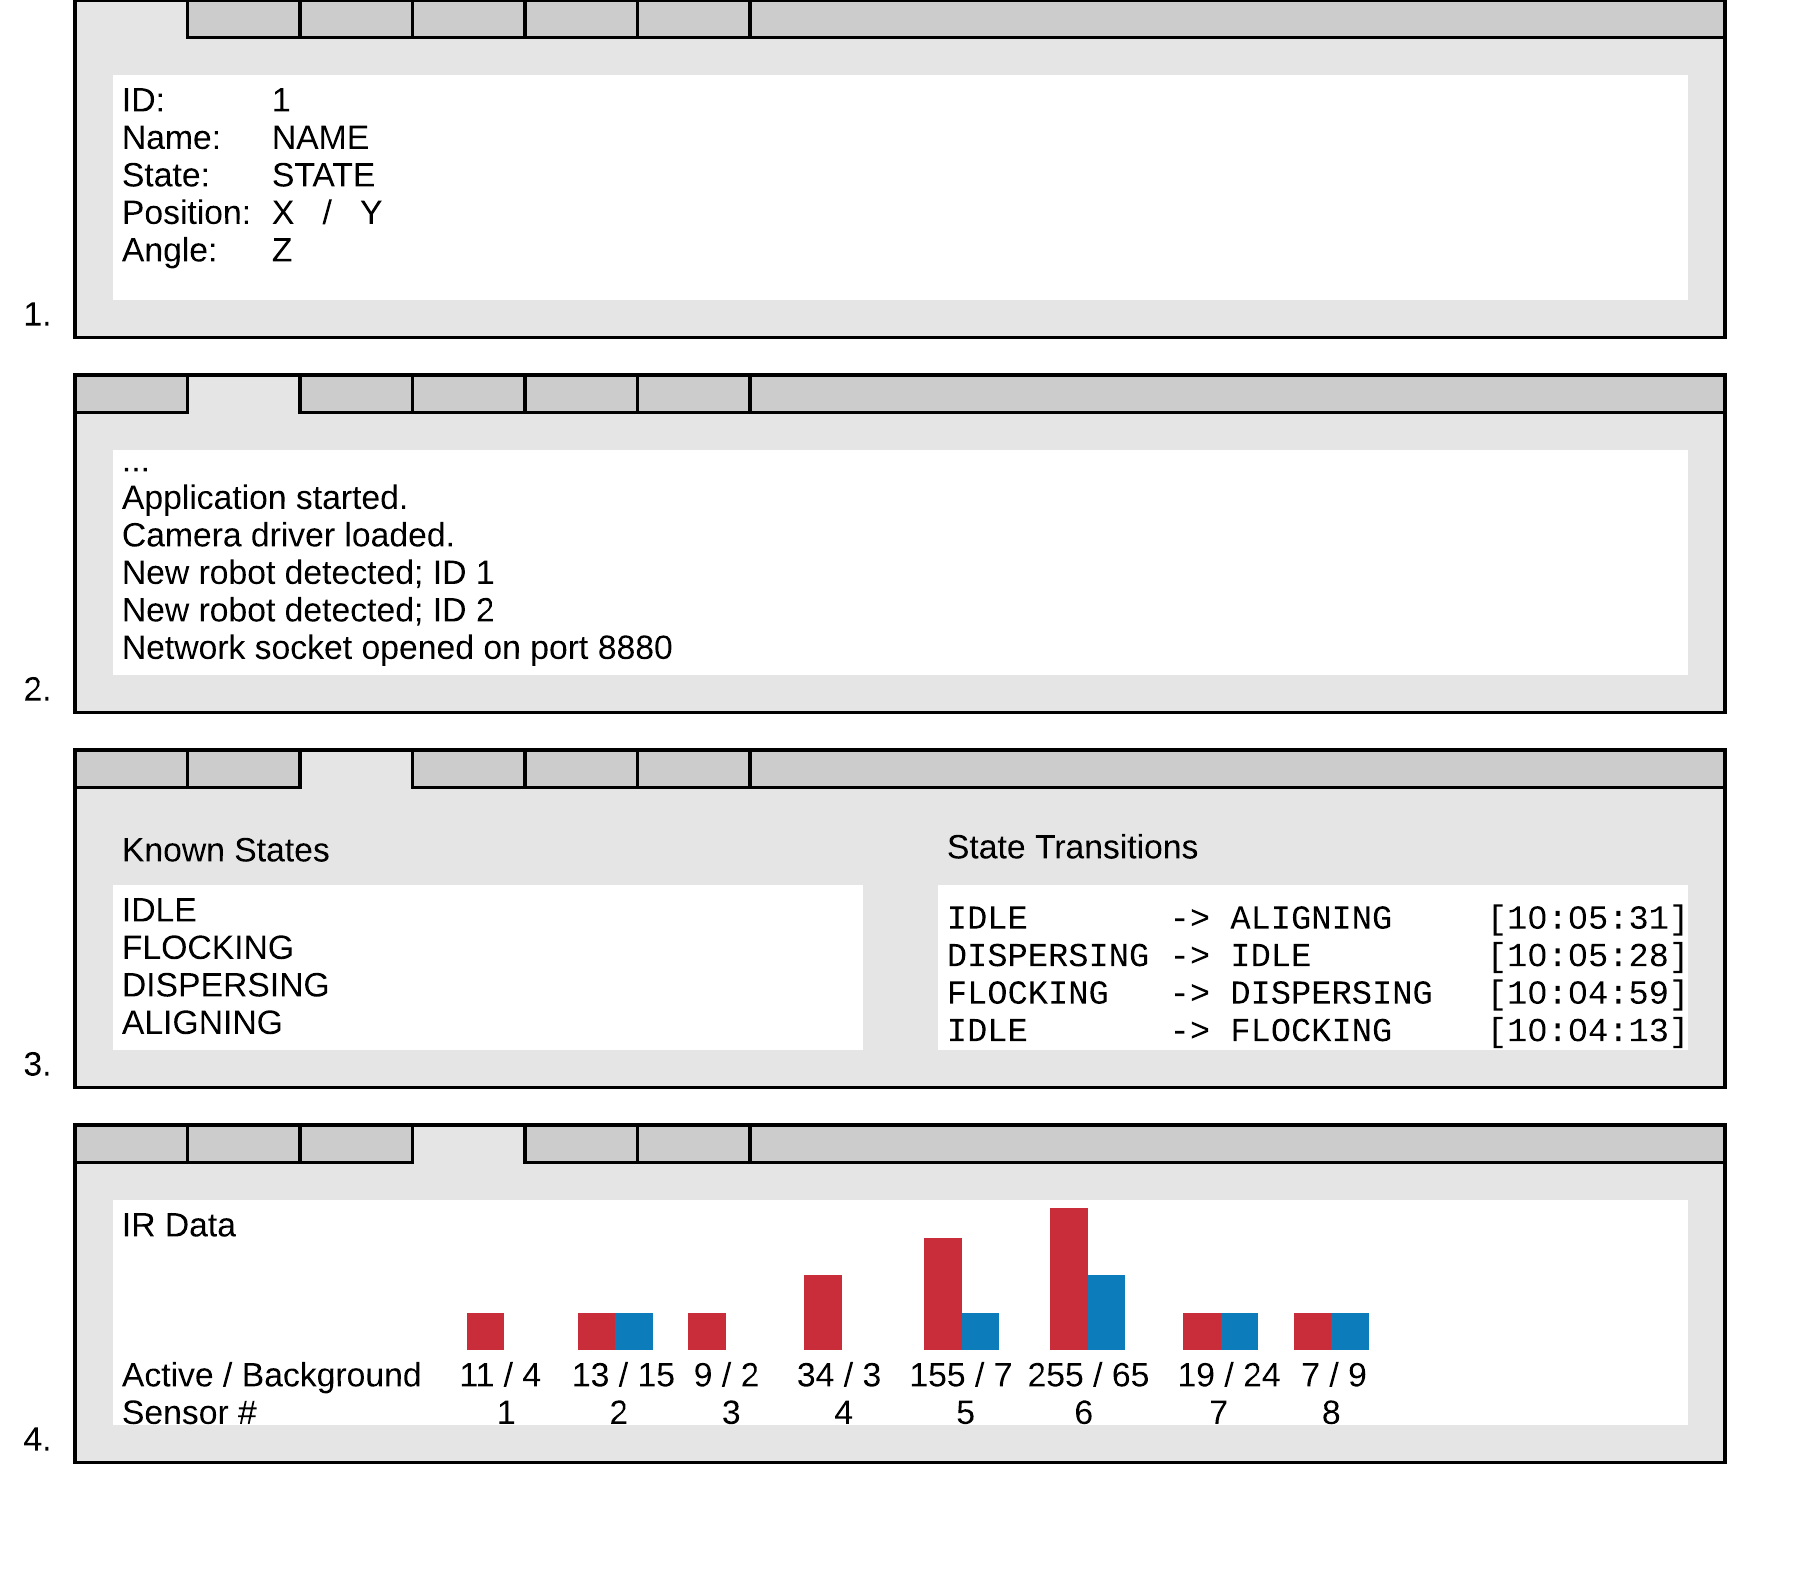
\includegraphics[scale=1]{Figures/DataPanelDesigns.png}
	\decoRule
	\caption[Data Panel Designs]{The initial UI designs created for some of the tabs within the data panel.}
	\label{fig:DataPanelDesigns}
\end{figure}

\begin{figure}
	\centering
	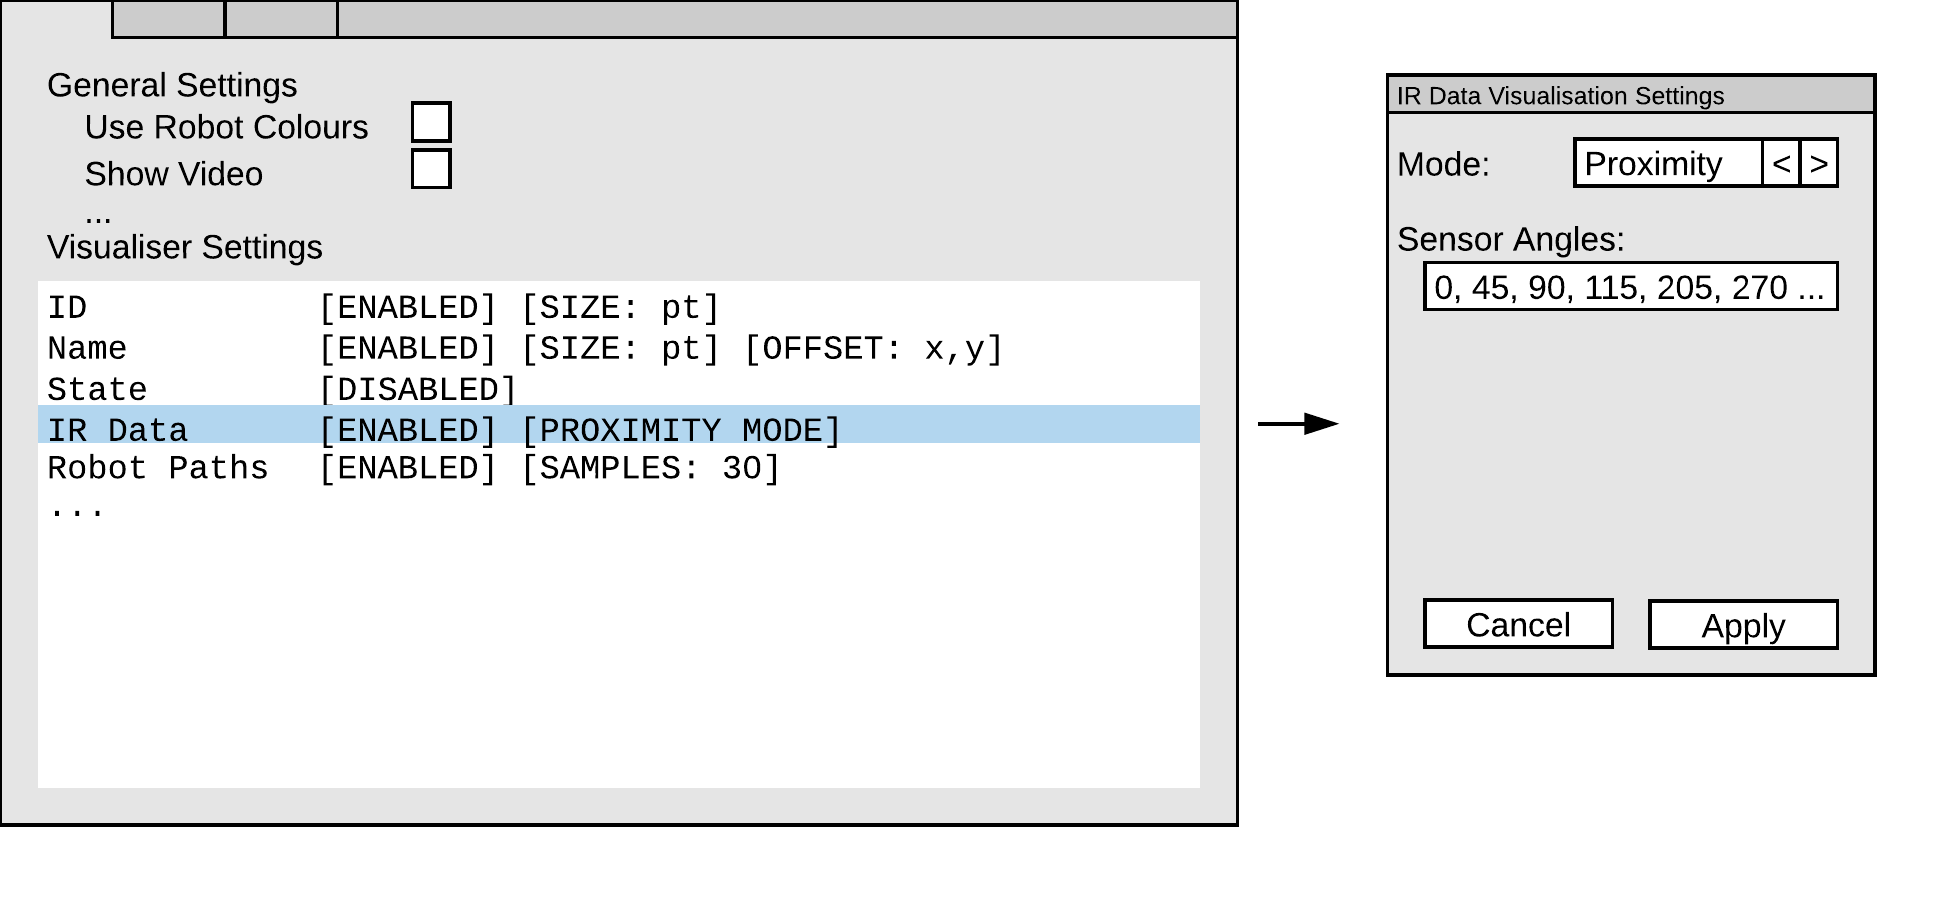
\includegraphics[scale=1]{Figures/VisualiserSettingsTabDesign.png}
	\decoRule
	\caption[Visualiser Settings Tab Design]{The initial UI design for the visualiser settings tab, and pop-up visualisation settings windows.}
	\label{fig:VisualiserSettingsTabDesign}
\end{figure}

\subsection{Data Visualisation Designs}

As well as designing layouts for some of the more complex individual UI elements, designs were also created for some of the graphical overlays that would be shown within the visualiser. The best way to visualise the data could not be determined prior to implementing the visualiser, hence a number of variations for the overlays of each type were generated. These could then be tried in practice to determine which were the most effective. Figure \ref{fig:OverlayDesigns} shows a selection of the overlay designs for the key data visualisation types, with the data visualisation shown in orange. Each row of the figure shows the visualisation design for a different type of data. The details of these designs are as follows.

\begin{description}
\item [Row 1.] Shows the representational 'robot' (a grey circle with an ArUco tag on top) with no overlay applied, for reference purposes. 

\item [Row 2.] Shows three options for the position overlay, including circular and square outline designs, and a filled circle design. It was thought that the filled circle might be easier for a user to see, but had the downside of obscuring the robot, whereas the outline designs might be more difficult to see due to the thinness of the lines.

\item [Row 3.] Shows three options for the direction overlay. The first uses a simple line on top of the robot, from its center outward, indicating its direction. The second develops on the first with an arrow, which might potentially add clarity, but would be more difficult to render at small sizes. The third also uses an arrow, rendered slightly away from the robot. This arrow could rotate to match the robots orientation, but maintain the same positional offset, or it could simply rotate with the robot about its center point. Offsetting the arrow makes the shape clearer as it does not overlap the robot, however in practice it could overlap other overlay elements, reducing the clarity of both. 

\item [Row 4.] Shows three options for the positioning of text overlays, including above and below the robot, and offset both vertically and horizontally. Text overlays are unlikely to be readable if rendered directly on top of the robot, and will always be prone to overlapping other elements if rendered with an offset. 

\item [Row 5.] Shows two possible IR data overlay designs. The first uses lines to display the sensor values, where the lines are oriented to face in the direction of the sensors, and their lengths vary with the relevant sensor value. If the lines were to very inversely with their related sensor values this could be used as an approximate proximity display. The second design shows a `heat map' style overlay, where the values of the sensors are indicated by boxes that change colour in relation to the relevant sensor value. 

\item [Row 6.] Shows three variations of the robot path overlay design, including smooth and stepped lines as well as solid and dotted variants. A smoother path line would likely require more data to be stored, which might be a disadvantage.
\end{description}

\begin{figure}
	\centering
	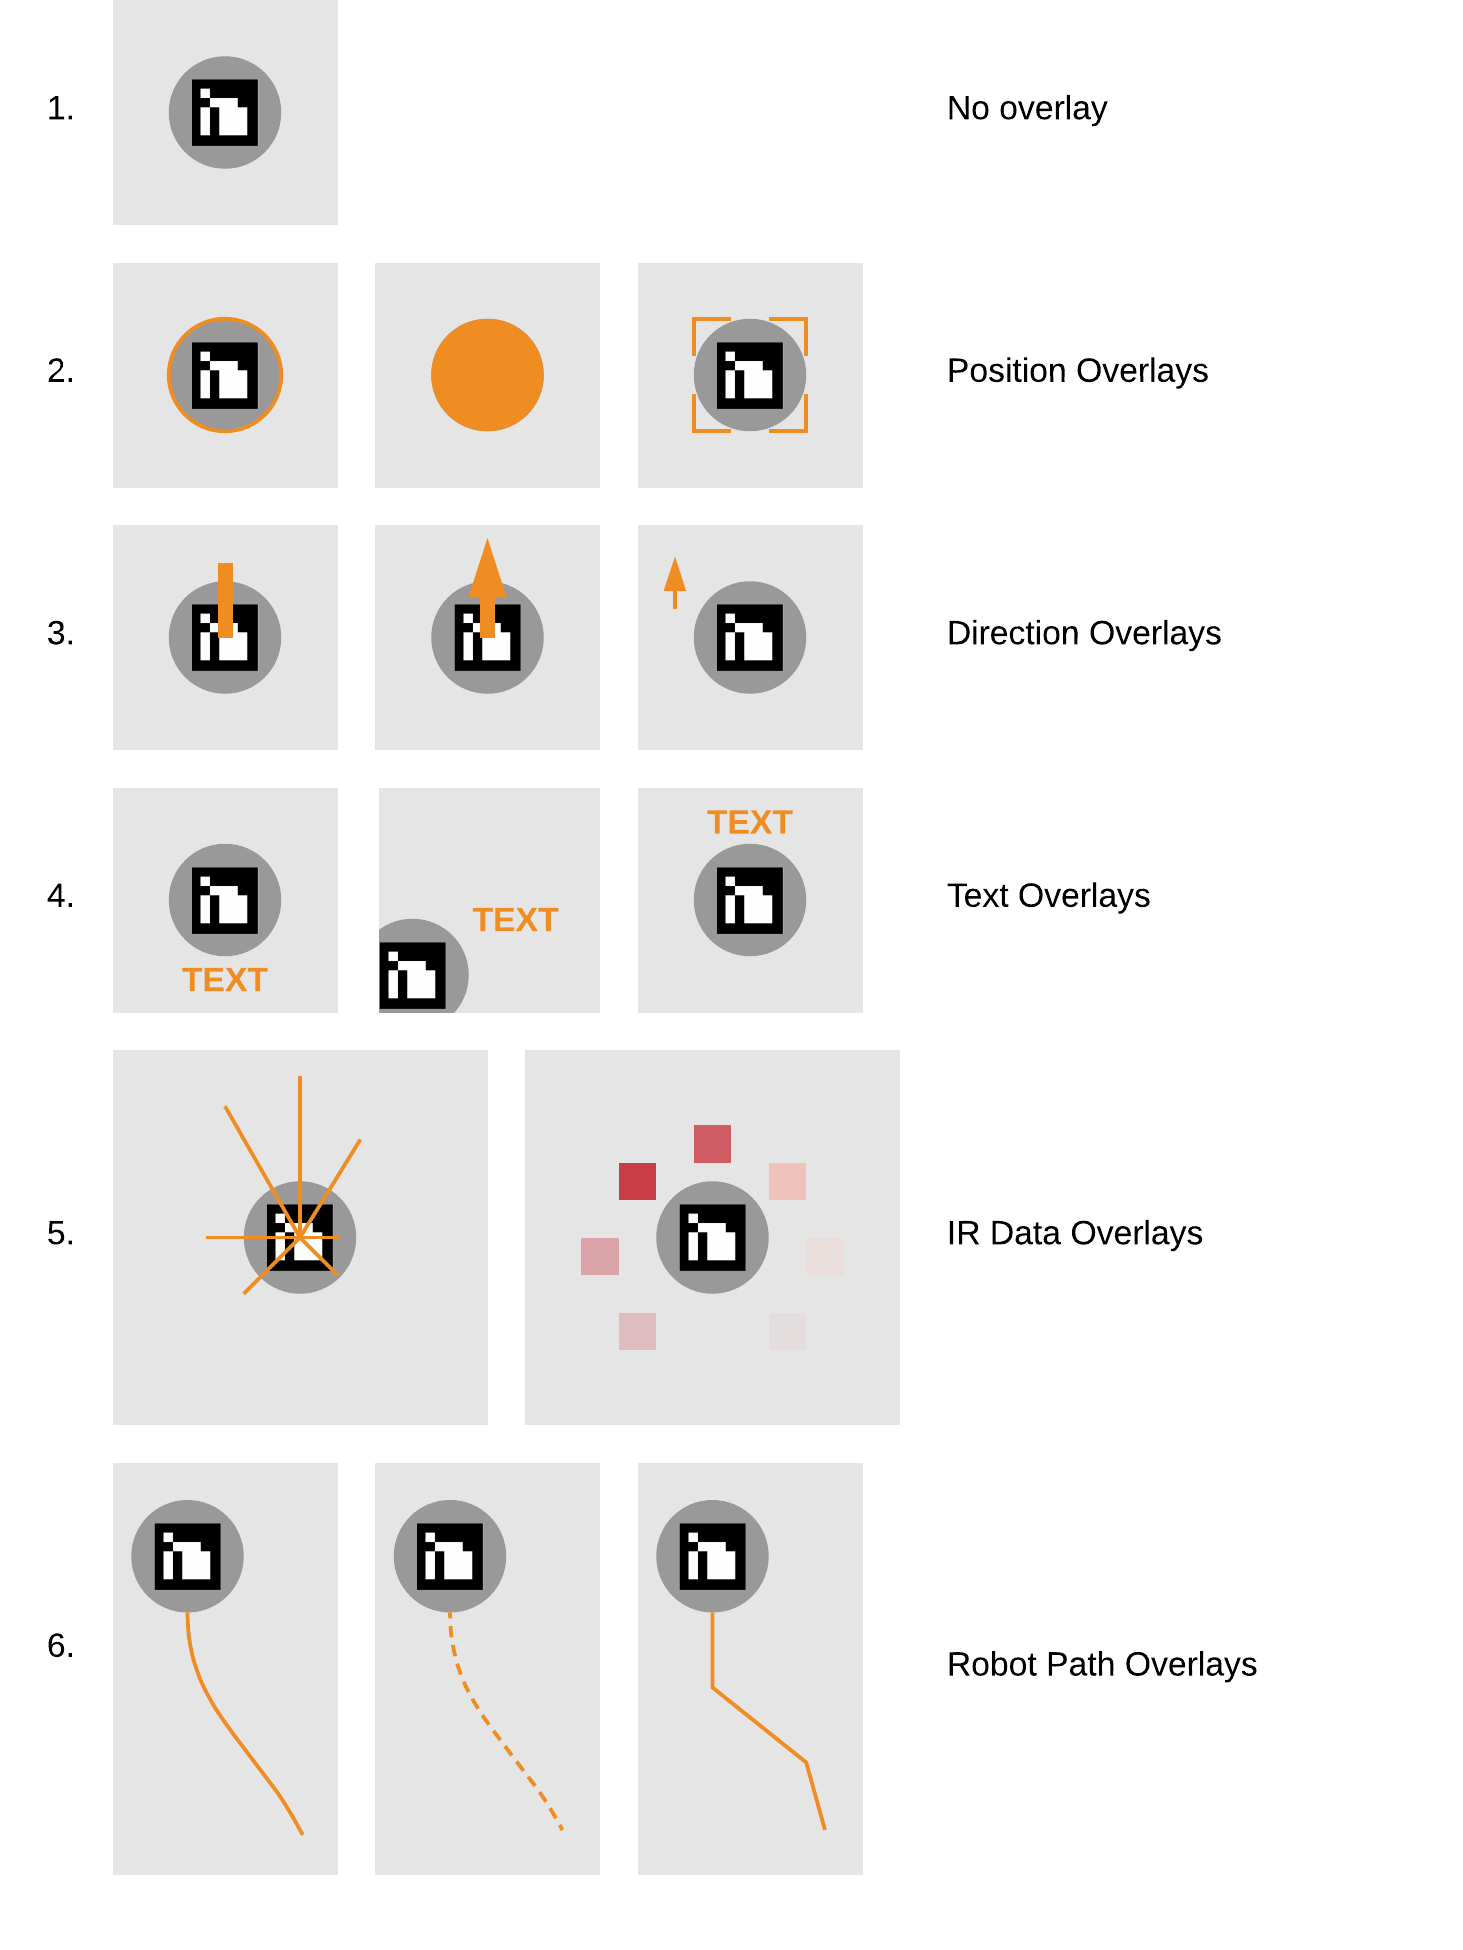
\includegraphics[scale=1]{Figures/OverlayDesigns.png}
	\decoRule
	\caption[Visualiser Overlay Designs]{A selection of the designs for visualiser overlays, for a number of data types.}
	\label{fig:OverlayDesigns}
\end{figure}

%----------------------------------------------------------------------------------------